%%%%%%%%%%
% [TODO] %
%%%%%%%%%%
% [ ] Mini-intro
% [ ] General methods
% [ ] Parlato2
% [ ] m-/ahpa/
% [ ] Mini-discussion

%%%%%%%%%%%%%%%%%%%%%%
% Chapter mini-intro %
%%%%%%%%%%%%%%%%%%%%%%

%%% Short BG


%%% Research question + alternatives


%%% Plan


%%%%%%%%%%%%%%%%%%%
% General methods % %
%%%%%%%%%%%%%%%%%%%

\section{General methods}
\subsection{ASR tools as models of perception}

\subsection{Anatomy of an ASR system}

\subsubsection{Corpora}
\paragraph{CSJ}
\begin{itemize}
\item General description (type of speech, number of speakers)
\item Alignment?
\item Phone set
\item ...
\end{itemize}

\paragraph{KCSS}
\begin{itemize}
\item General description (type of speech, number of speakers)
\item Alignment?
\item Phone set
\item ...
\end{itemize}

\subsubsection{Features}
\begin{itemize}
\item What are MFCCs
\item VTLN and CMVN
\item Pitch
\item LDA?
\item ...
\end{itemize}

\subsubsection{Acoustic model}
\begin{itemize}
\item Monophone model - also, why?
\item Number of gaussians
\item Number of states
\item ...
\end{itemize}
    
\subsubsection{Language models}
\begin{itemize}
\item WFSTs
\item Words \& phones 
\item n-grams
\item ...
\end{itemize}

\subsubsection{Decoding}
\begin{itemize}
\item Lattice generation
\item Acoustic and LM scores 
\item nbest
\item CTM
\item ...
\end{itemize}

\subsection{Assessing native performance}
\subsubsection{Lexicon-based decoding}
\subsubsection{Phonetic-based decoding}

\subsection{Human-model comparisons} \label{3-methods_comparison}
\subsubsection{Simulations}
\subsubsection{Data analysis: ABC easy as 123} \label{3-methods_comparison_ABC}
\paragraph{Reasoning}
\paragraph{Model selection}
\paragraph{Parameter tuning}

%%%%%%%%%%%%
% Parlato2 %
%%%%%%%%%%%%

\section{{\color{red}Parlato-hmm}} \label{3-parlato-hmm}
\subsection{Introduction}
\subsection{Methods}
\subsubsection{Stimuli}
We used the same stimuli as in section \ref{2-parlato}. As a reminder, a native French speaker recorded 54 items with the structure $V_{1}C_{1}C_{2}V_{2}$, with $V_{1}$ and $V_{2}$ vowels from the set \{/a/, /i/, /u/\}, and $C_{1}C_{2}$ a cluster from the set \{/bg/, /bn/, /db/, /dg/, /gb/, /gn/\} (e.g. /abgi/).

\subsubsection{Language models}
In order for the decoding task to be analogous to the experiment described in section \ref{2-parlato_per}, trial-specific language models were constructed, as shown in Figure \ref{fig:parlato_G}. Thus, when decoding a $V_{1}C_{1}C_{2}V_{2}$ stimulus, the perception model is only given the possibility to transcribe it as $V_{1}C_{1}(V_{3})(SIL)C_{2}V_{2}$, where phones between parentheses are optional and $V_{3}$ is from the set \textipa{/a, e, i, o, u/}. In this section our language model is only used to constrain the list of possible outputs from decoding; one output is not more probable than another based on the language models alone. Therefore, here we use a null language model, meaning that the quality of the epenthesized vowels will only be determined by acoustic and duration matches.

\begin{figure}[htb]
\centering
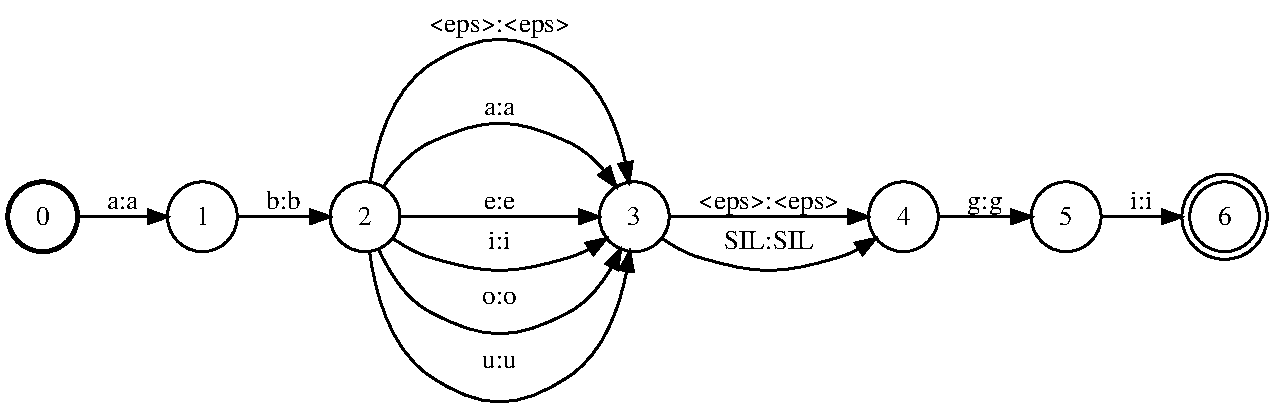
\includegraphics[width=0.8\linewidth]{chapter03/parlato_hmm_Gfst.pdf}
\caption{Constrained language model used for decoding the stimulus \textipa{/abgi/}. Nodes in the graph represent states, edges represent transitions between states (here: phonemes). The lack of weights on edges issued from a same node (e.g., between states 2 and 3) indicates that path selection is entirely decided by acoustic scores when decoding experimental items. An optional silence can be inserted by the model between states 3 and 4.}
\label{fig:parlato_G}
\end{figure}

\subsubsection{Data analysis}
Using scores from our model, we simulated the perceptual experiment described in section \ref{2-parlato_per}, as explained in section \ref{3-methods_comparison}. %In order to assess the role of duration on the choice of epenthetic vowel quality, we inferred the \textit{a posteriori} distributions of the weights given to acoustic model, language model, and duration scores in {\color{red}equation \ref{}}, using ABC. The following aggregated data were used as summary statistics:

% \begin{itemize}
% \item \%none: Proportion of ``none'' responses (no epenthesis)
% \item \%$V_{1}\underline{\vee}V_{2}$: Proportion of vowel copy where the epenthesized vowel shares the quality of either $V_{1}$ or $V_{2}$, with $V_{1} \neq V_{2}$)
% \item \%$V_{1}\land V_{2}$: Proportion of vowel copy where the epenthesized vowel shares the quality of both $V_{1}$ and $V_{2}$, with $V_{1} = V_{2}$)
% \item \%default: Proportion of default \textipa{/u/}-epenthesis over all trials
%   \item \%coronal: Proportion of \textipa{/o/}-epenthesis following coronal consonants over all trials with clusters containing coronal consonants 
% \end{itemize}  
\subsection{Results}
\subsection{Discussion}


%%%%%%%%%%%%
% m-/ahpa/ %
%%%%%%%%%%%%

\section{{\color{red}m-/ahpa/ + Parlato-lms}} \label{3-m-ahpa}
\subsection{Introduction}
\subsection{Methods}
\subsubsection{Stimuli}
We used the same stimuli as in section \ref{2-ahpa}. As a reminder, we recorded 3 speakers producing disyllabic $V_{1}C_{1}C_{2}V_{1}$ and trisyllabic $V_{1}C_{1}V_{2}C_{2}V_{1}$, with $V_{1}$ a flanking vowel in the set \textipa{/a, e, i, o, u/}, $C_{1}$ \textipa{/h/} or /k/, and $C_{2}$ a fixed consonant, /p/ (e.g, \textipa{/ahpa/}, \textipa{/ahapa/}). By splicing the disyllabic natural control items (e.g., \textipa{/ahpa/}), we obtained disyllabic spliced control items (e.g., \texorpdfstring{\textipa{/ah\textsubscript{a}pa/}}{}), disyllabic spliced test stimuli (e.g., \texorpdfstring{\textipa{/ah\textsubscript{u}pa/}}{}), and trisyllabic spliced fillers (e.g., {\textipa{/ahapa/}). Therefore, within each speaker, all stimuli of the same structure (in our example, \textipa{/ah($V$)pa/} items) are acoustically identical on their flanking vowels.

\subsubsection{Language models}
In this section, we investigate the type of phonotactic information used by Japanese listeners when perceiving foreign speech that does not conform to native phonotactics. We test 5 types of language models (LM): 
\begin{enumerate}
    \item A null language model (0P-LM), which implies that listeners base their decoding of consonant clusters on phonetics alone, without using information on phonotactics (similar to that used in section \ref{3-parlato2})
    \item A phone-unigram language model (1P-LM), which implies that listeners do not take neighbouring phonemes into consideration when decoding the consonant clusters
    \item An online phone-bigram language model (2PO-LM), which implies that listeners decode the clusters as they hear them (decoding is done from the start of the item)
    \item A retro phone-bigram language model (2PR-LM), which implies that listeners decode the clusters based on the most recent information (decoding is done from the end of the item)
    \item A batch phone-bigram language model (2PB-LM), which implies that listeners decode the item considering the entire structure, with bigrams %use bigram transitional probabilities from the entire cluster, in order to find a global optimal transcription
    \end{enumerate}

    \begin{figure}[htb]
    \centering
    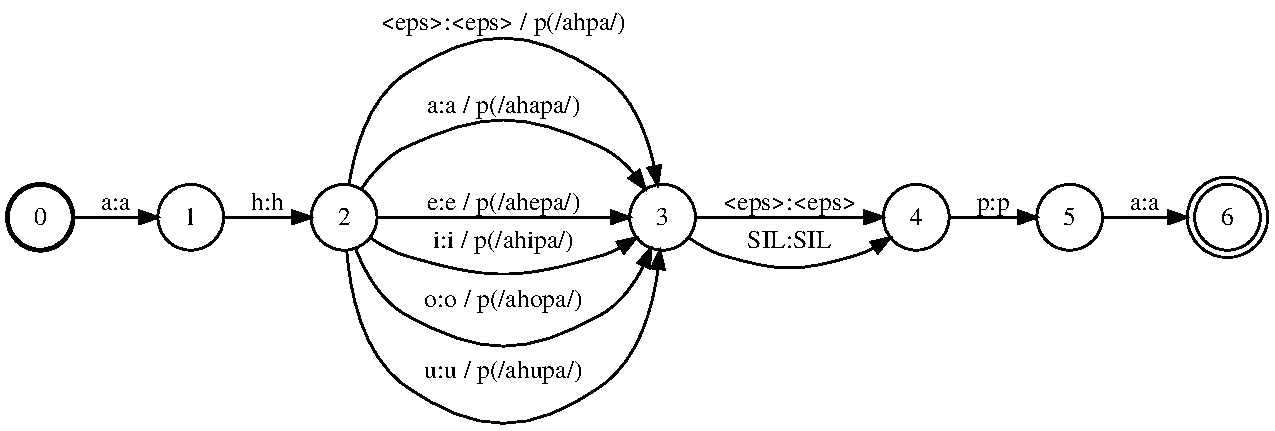
\includegraphics[width=0.8\linewidth]{chapter03/m-ahpa_Gfst.pdf}
    \caption{Constrained language model used to test the models (here: LM for \textipa{/ahpa/} trials). Nodes in the graph represent states, weighted edges represent transitions between states (here: phonemes). When relevant, weighted edges are labeled with the probability to choose that edge when decoding, which affects the final language model score of each possible path. These scores are then combined with acoustic and duration scores when decoding experimental items.}
    \label{fig:m-ahpa_G}
\end{figure}
\subsubsection{Data analysis}
\subsection{Results}
\subsection{Discussion}

%%%%%%%%%%%%
% k-epenth %
%%%%%%%%%%%%

\section{{\color{red}k-epenth}} \label{3-k-epenth}
\subsection{Introduction}
\subsection{Methods}
\subsubsection{Stimuli}

\subsubsection{Procedure}

\subsubsection{Data analysis}
\subsection{Results}
\subsection{Discussion}
%%%%%%%%%%%%%%%%%%%%%%%%%%%
% Chapter mini-discussion %
%%%%%%%%%%%%%%%%%%%%%%%%%%%
\section{Conclusions}
%%% Summary

%%% Short discussion

%%% Limitations

%%% Conclusions